\scanpage{69}\mspage{68}
% First paragraph; the two additions and their distinct connecting strokes are kept in this local group.
% figure R1-F1
\figure{%
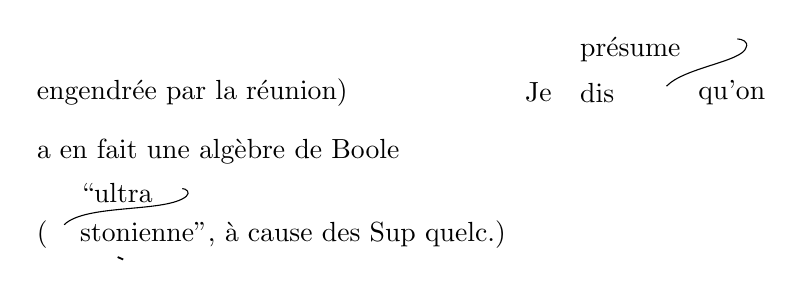
\begin{tikzpicture}[x=1cm,y=1cm]
  \node[anchor=west] at (0,1.8) {engendrée par la réunion)};
  \node[anchor=west] at (6.2,1.8) {Je};
  \node[anchor=west] at (6.9,1.8) {\deleted{dis}};
  \node[anchor=west] at (8.4,1.8) {qu'on};
  \node[anchor=west] at (6.9,2.35) {\inserted{présume}};
  \draw (8.12,1.88) .. controls (8.35,2.12) and (9.08,2.19) .. (9.13,2.37) .. controls (9.17,2.45) and (9.07,2.48) .. (9.02,2.48);
  \node[anchor=west] at (0,1.05) {a en fait une algèbre de Boole};
  \node[anchor=west] at (0,0) {(};
  \node[anchor=west] at (0.55,0) {stonienne'', à cause des $\mathrm{Sup}$ quelc.)};
  \node[anchor=west] at (0.55,0.53) {\inserted{``ultra}};
% Detached short stroke below stonienne; no function is assigned.
  \draw[line width=0.65pt] (1.15,-0.29)--(1.22,-0.32);
  \draw (0.47,0.12) .. controls (0.74,0.39) and (1.76,0.27) .. (2.02,0.48) .. controls (2.08,0.53) and (2.02,0.58) .. (1.97,0.58);
\end{tikzpicture}%
}
% slanted left margin note
\margin{Cela sera valable dans ``le cas ensembliste'', et en tous cas dans les exemples types, donnés \deleted{\unsure{tout}} au début, en termes d'un $E$ (top. ou mesurable), alors $\Sigma$ s'identifie à l'ens des parties de $E$, et \unsure{on trouve|on trouvera|on retrouve} le compactifié de \unsure{Stone} de $E_{\mathrm{disc.}}$ Dans le cas qui vient, \unsure{je} \unsure{ne vois} comment \unsure{prouver}, pour trois supports
\[P,Q,R\quad P\wedge(Q\vee R)=\unsure{\{|(}(P\wedge Q)\vee(P\wedge R)\unsure{\}|.|,|)}\]}

\deleted{Il faudra y revenir}

\unsure{Donc} les supports \unsure{s'identifient|s'identifieraient} aux \unsure{Parties|Partie} à la fois ouvertes et fermées du spectre, qui serait un espace \deleted{\unsure{to|tot}}\unsure{cpct|cpt|compact} \deleted{\unsure{tot}} \unsure{disconnexe} ultra.stonien.

L'involution correspond au passage au complémentaire.

% Construction paragraph with the two insertion leaders; words occur once.
% figure R1-F2
\figure{%
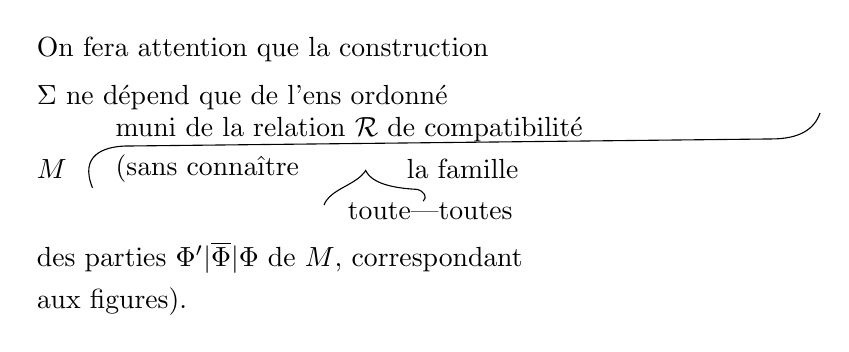
\begin{tikzpicture}[x=1cm,y=1cm]
  \node[anchor=west] at (0,2.0) {On \unsure{fera} attention que la construction};
  \node[anchor=west] at (0,1.38) {$\Sigma$ ne dépend que de l'ens ordonné};
  \node[anchor=west] at (0,0.48) {$M$};
  \node[anchor=west] at (1.0,0.48) {(sans connaître};
  \node[anchor=west] at (4.7,0.48) {la famille};
  \node[anchor=west] at (1.0,0.98) {\inserted{muni de la relation $\mathcal R$ de compatibilité}};
  \draw (0.83,0.24) .. controls (0.66,0.66) and (0.98,0.76) .. (1.24,0.77) -- (9.45,0.86) .. controls (9.82,0.86) and (10.00,0.99) .. (10.07,1.19);
  \node[anchor=west] at (3.95,-0.06) {\inserted{\unsure{toute|toutes}}};
  \draw (3.77,0.02) .. controls (3.85,0.23) and (4.18,0.27) .. (4.30,0.46) .. controls (4.39,0.26) and (4.77,0.23) .. (4.95,0.22) .. controls (5.04,0.20) and (5.09,0.12) .. (5.03,0.07);
  \node[anchor=west] at (0,-0.65) {des parties $\unsure{\Phi'|\overline\Phi|\Phi}$ de $M$, correspondant};
  \node[anchor=west] at (0,-1.20) {aux figures).};
\end{tikzpicture}%
}
En effet, en termes de $(M,\leq,R)$, le cosupport d'une partie $M'$ de $M$ est défini par
\[
\operatorname{cosup}_M(M')=\{\,x\in M\mid(x,x')\in\mathcal R\quad\forall x'\in\unsure{M'|M''}\,\}
\]
% Slanted bottom margin note and its long attached rule; no arrowhead is supplied.
% figure R1-F3
\figure{%
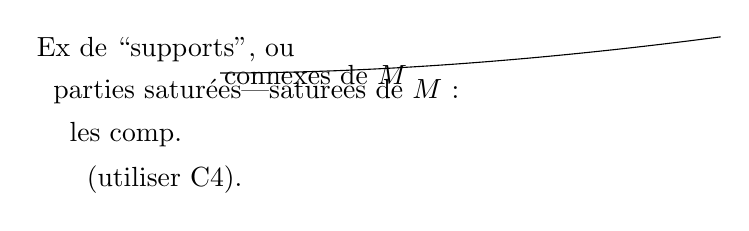
\begin{tikzpicture}[x=1cm,y=1cm]
\begin{scope}[rotate=21]
  \node[anchor=west] at (0,0) {\uline{Ex} de ``supports'', ou};
  \node[anchor=west] at (0,-0.58) {parties \unsure{saturées|saturees} de $M$ :};
  \node[anchor=west] at (0,-1.16) {les comp.};
  \node[anchor=west] at (2.10,-1.16) {connexes de $M$};
  \node[anchor=west] at (0,-1.77) {(utiliser C4).};
  \draw (2.18,-1.16) .. controls (4.23,-1.95) and (6.45,-2.57) .. (8.28,-3.01);
\end{scope}
\end{tikzpicture}%
}
